\chapter{Memoria centrale}
\section{Introduzione}

Abbiamo visto che i moderni SO tentano di massimizzare l'uso delle risorse della macchina, e in primo luogo l'utilizzo della CPU.
\begin{itemize}
    \item Questo si ottiene mediante le due tecniche fondamentali del multi-tasking e del time-sharing, che richiedono di tenere in memoria primaria contemporaneamente più processi attivi.
    \item Il SO deve decidere come allocare lo spazio di RAM tra i
    processi attivi, in modo che ciascun processo sia pronto per
    sfruttare la CPU quando gli viene assegnata.
\end{itemize}

Supponiamo però che, ad un certo punto, la RAM sia \textbf{completamente} occupata da 3 processi utente, P1, P2, P3 (per semplicità assumiamo che a tutti i processi venga assegnata una porzione di RAM della stessa dimensione).

\qs{}{Un nuovo processo P4 viene fatto partire, è immediatamente pronto per usare la CPU, ma non c'è più spazio per caricare il suo codice in RAM, che si può fare?}

\begin{itemize}
    \item Ovviamente si potrebbe aspettare la terminazione di uno dei
    3 processi già in RAM, ma supponiamo che uno dei tre
    processi (diciamo P2) sia temporaneamente in attesa di
    compiere una lunga operazione di I/O (per cui non userà la
    CPU a breve).
\end{itemize}

Il SO potrebbe decidere di spostare temporaneamente P2 sull'hard disk per far posto a P4, che così può concorrere all'uso della CPU.
\dfn{Swapping}{
    \begin{itemize}
        \item Che cosa viene spostato sull'hard disk? L'immagine di P2: il
        codice (anche se, come capiremo meglio più avanti, questo
        si può anche evitare), i dati e lo stack del processo.
        \item Dopo un po' P1 termina e libera una porzione di RAM. Il
        SO potrebbe riportare P2 in RAM (ma ora nello spazio che
        era stato inizialmente assegnato a P1).
    \end{itemize}
    
    Questa tecnica viene chiamata \textit{swapping} (avvicendamento di processi). L'area del disco in cui il SO copia temporaneamente un processo viene detta area di \textit{swap}.
}
\qs{}{
Lo \textit{swapping} è raramente usato nei moderni sistemi
operativi perché troppo inefficiente, ma l'esempio mette in
luce un problema fondamentale nella gestione della
memoria primaria: P2 contiene istruzioni che usano indirizzi
di memoria primaria: funziona ancora correttamente
quando viene spostato da un'area di RAM ad un'altra?
}
\begin{figure}[h]
    \centering
    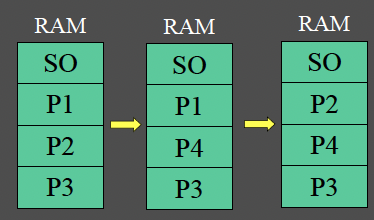
\includegraphics[width=0.5\linewidth]{images/table_swap.png}
\end{figure}
 
\begin{figure}[h]
    \centering
    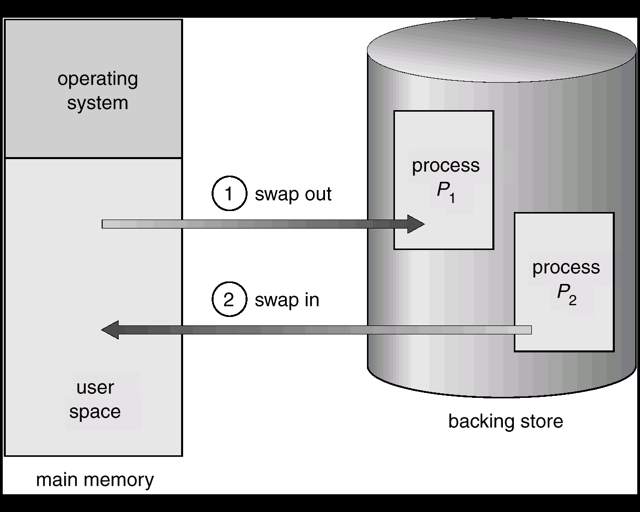
\includegraphics[width=0.5\linewidth]{images/swap-mem.png}
    \caption{Swap mem}
    \label{fig:swap-mem}
\end{figure}
Perché un programma possa essere \textbf{eseguito}, il suo codice deve trovarsi in \textbf{memoria} \textbf{primaria} (ma rivedremo questa affermazione quando parleremo della memoria virtuale)
Quindi, quando il SO riceve il \textbf{comando} di esecuzione di un programma, deve recuperare il codice del programma dalla memoria secondaria, e decidere in quale porzione della memoria primaria sistemarlo. ossia, a partire da quale indirizzo di RAM.

\section{Binding (associazione degli indirizzi)}
Un programma sorgente usa (tra l'altro) dati (variabili) e
istruzioni di controllo del flusso di computazione.
\begin{itemize}
    \item Quando il programma viene compilato e caricato in
    Memoria Primaria (MP) per essere eseguito, ad ogni
    variabile è associato l'\textbf{indirizzo} di una locazione di
    memoria che ne contiene il valore.
    \item Alle istruzioni di controllo del flusso di esecuzione del
    programma (ossia i salti condizionati e incondizionati) è
    associato l'indirizzo di destinazione del salto.
    \item L'operazione di associazione di variabili e istruzioni agli
    indirizzi di memoria è detta \textit{binding degli indirizzi}.
\end{itemize}

In altre parole, ad ogni variabile dichiarata nel programma viene fatto corrispondere l'indirizzo di una cella di memoria di RAM in cui verrà memorizzato il valore di quella variabile.
\begin{itemize}
    \item L'accesso alla variabile, in lettura e scrittura, corrisponde
    alla lettura e scrittura della cella di memoria il cui indirizzo
    è stato "legato" (con l'operazione di binding) alla variabile.
    \item Le istruzioni di salto, che permettono di implementare
    costrutti come \textit{if-then-else}, \textit{while}, ecc., sono associate agli
    indirizzi in RAM dove si trova l'istruzione con cui prosegue
    l'esecuzione del programma se il salto viene eseguito.
\end{itemize}

Ad esempio, un'istruzione C come:
\begin{verbatim}
counter = counter + 1;
\end{verbatim}
alla fine diventerà qualcosa del tipo:
\begin{verbatim}
load(R1, 10456)
Add(R1, #1);
store(R1, 10456)
\end{verbatim}
10456 è l'indirizzo della cella di memoria che contiene il
valore della variabile \textit{counter}. L'indirizzo 10456 è stato
associato alla variabile \textit{counter} durante la fase di binding
degli indirizzi.


Analogamente, un'istruzione C come:
\begin{verbatim}
while (counter <= 100) counter++;
\end{verbatim}
alla fine diventerà qualcosa del tipo:
\begin{verbatim}
100FC jgt(R1, #100, 10110) // jump if greater than
10100 load(R1, 10456)
10104 Add(R1, #1)
10108 store(R1, 10456)
1010C jmp(100FC)
10110 ... ...
\end{verbatim}

Rispetto all'indirizzo di istruzione del salto stesso, il \textit{while} della slide precedente potrebbe anche essere tradotto in assembler così:
\begin{verbatim}
100FC jgt(R1, #100, 00014) // jump if greater than
10100 load(R1, 10456)
10104 Add(R1, #1)
10108 store(R1, 10456)
1010C jmp(100FC)
10110 ... ...
\end{verbatim}

Perché un programma sorgente
possa essere eseguito deve passare
attraverso varie fasi. Il binding degli indirizzi avviene
in una di queste fasi:
\begin{itemize}
    \item compilazione
    \item caricamento (in RAM)
    \item esecuzione
\end{itemize}

\begin{figure}[h]
    \centering
    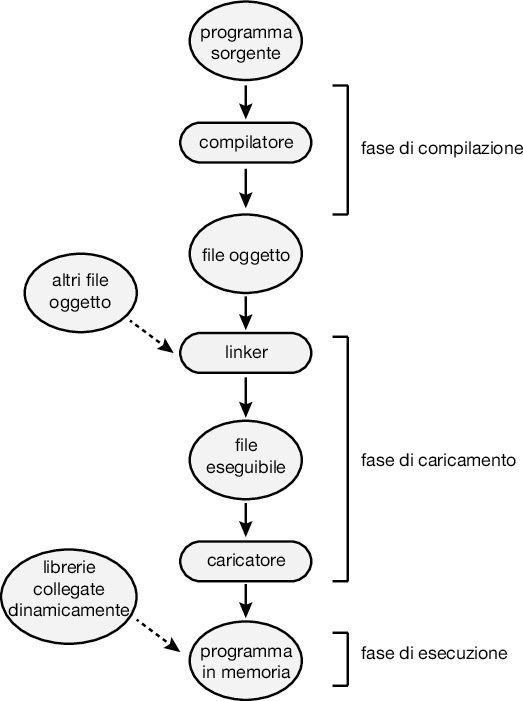
\includegraphics[width=0.25\linewidth]{images/process_compilation.png}
    \caption{Processo di compilazione da programma sorgente}
    \label{fig:compilate-process}
\end{figure}

\subsection{Quando?}
\begin{enumerate}
    \item In fase di Compilazione 
        \begin{itemize}
        \item viene generato codice assoluto o statico.
        \item Il compilatore deve conoscere l'indirizzo della cella di
        RAM a partire dal quale verrà caricato il programma,
        in modo da effettuare il \textit{binding} degli indirizzi
        (che avviene, appunto, in fase di compilazione).
        \item Se il SO deve scaricare temporaneamente il processo
        che usa quel codice in Memoria Secondaria (MS), come
        nell'esempio visto a inizio capitolo, quando lo ricarica
        in RAM deve rimetterlo esattamente dove si trovava
        prima. (Oppure?)
        \end{itemize}
    \item  In fase di caricamento in RAM
        \begin{itemize}
        \item Viene generato codice staticamente rilocabile.
        \item Il compilatore associa ad istruzioni e variabili degli
        indirizzi relativi rispetto all'inizio del programma,
        che inizia da un ipotetico indirizzo 0 virtuale.
        \item Gli indirizzi assoluti finali vengono generati in fase di
        caricamento del codice in Memoria Primaria (MP) in base all'indirizzo di
        MP a partire dal quale è caricato il codice.
        \item Il binding degli indirizzi, quindi, avviene in fase di
        caricamento del programma in RAM: se il processo che
        usa quel codice viene tolto dalla RAM, si può caricarlo
        in una posizione diversa solo rieffettuando la fase di
        caricamento (ma è più efficiente che ricompilare tutto).
        \end{itemize}
    \item In fase di esecuzione
        \begin{itemize}
        \item Viene generato codice dinamicamente rilocabile.
            \item Il codice in esecuzione usa sempre e solo indirizzi
            relativi.
            \item La trasformazione di un indirizzo relativo in uno
            assoluto viene fatta nell'istante in cui viene eseguita
            l'istruzione che usa quell'indirizzo.
            \item È necessario un opportuno supporto hardware per realizzare
            questo metodo senza perdita di efficienza.
            \item Si parla di \textit{binding dinamico} degli indirizzi.
            \item In opportuno registro di rilocazione viene usato per trasformare un indirizzo relativo nel corrispondente indirizzo assoluto durante l’esecuzione delle istruzioni.
            \item Il registro di rilocazione contiene l’indirizzo di partenza dell’area di RAM in cui è caricato il programma in esecuzione.
            \item La memory management Unit (MMU) si occuperà di trasformare gli indirizzi relativi in assoluti, usando il registro di rilocazione, per accedere alle celle di RAM indirizzate dalle istruzioni
            \item Lo spostamento del processo da un area all’altra della MP è realizzabile senza problema.
            \item Il SO deve solo ricordarsi dell’indirizzo della locazione di MP a partire dalla quale è memorizzato il processo
        \end{itemize}
        \nt{Per spostare i programmi da un’area di RAM ad un’altra ora basta cambiare l’indirizzo scritto nel registro di rilocazione (fig. 9.5 modificata)}
\end{enumerate}

\section{Spazio degli indirizzi (Logici e Fisici)}
Consideriamo codice dinamicamente rilocabile (d’ora in poi faremo sempre riferimento a codice dinamicamente rilocabile, se non indicato diversamente). Ogni indirizzo usato nel codice è riferito ad un ipotetico indirizzo 0 (zero): l’indirizzo della prima istruzione di cui è formato il codice.

Gli indirizzi utilizzati in un programma possono essere:
\begin{itemize}
    \item l'indirizzo di una cella di memoria che contiene una variabile
    \item l'indirizzo di un'istruzione di salto
\end{itemize}

Questi indirizzi rientrano nello \textbf{spazio di indirizzamento logico o virtuale}, che va da 0 all'ultima cella di memoria occupata. Quando il codice viene caricato in RAM, gli \textbf{indirizzi logici} generati dalla CPU vengono trasformati in \textbf{indirizzi fisici} attraverso il registro di rilocazione, permettendo di indirizzare correttamente la memoria fisica (RAM).

Lo \textbf{spazio di indirizzamento fisico} è l'insieme degli indirizzi fisici che dipende dall'area di memoria dove il sistema operativo ha caricato il programma.

Per i programmi con codice rilocabile dinamicamente esistono due tipi di indirizzi:
\begin{itemize}
    \item Indirizzi logici, che vanno da $0$ a $max$
    \item Indirizzi fisici, che vanno da $r+0$ a $r+max$, dove $r$ è l'indirizzo iniziale della RAM in cui il programma è caricato
\end{itemize}

Gli indirizzi logici vengono sempre mappati in indirizzi fisici per accedere correttamente alla RAM.

Le espressioni \textbf{spazio di indirizzamento logico} e \textbf{spazio di indirizzamento fisico} si riferiscono principalmente all'architettura di un sistema, non a singoli programmi.

Consideriamo un computer con un massimo di 64 Kbyte di RAM, ovvero 65536 byte. In questo contesto, possiamo dire che:
\begin{enumerate}
    \item Il computer può indirizzare $2^{16}$ byte di RAM.
    \item Gli indirizzi dei byte della RAM vanno da 0000 a FFFF in esadecimale (da 0 a $2^{16} - 1$).
    \item L'indirizzo di ciascun byte della RAM è rappresentato da 16 bit.
\end{enumerate}

Pertanto, lo \textbf{spazio di indirizzamento fisico} di questo computer è scritto su 16 bit e va da 0000 a FFFF, con una dimensione di 64 Kbyte.

Se un compilatore genera codice dinamicamente rilocabile e utilizza 12 bit (\textbf{perchè 12?}) per scrivere un indirizzo logico, lo \textbf{spazio di indirizzamento logico} di un programma sarà di massimo $2^{12}$ byte, ovvero 4 Kbyte. Nessun programma potrà superare questo limite, anche se può usare uno spazio logico inferiore.

Quindi, possiamo dire che lo spazio di indirizzamento logico dei programmi di questo computer è scritto su 12 bit, va da 0000 a 0FFF (esadecimale) ed è di 4 Kbyte.

In seguito, quando parleremo di spazi di indirizzamento, ci riferiremo a quelli dell'intera macchina, e non a quelli dei singoli programmi. Tuttavia, è possibile considerare un programma che occupa tutto lo spazio di indirizzamento logico della macchina.

\qs{}{Ha senso che la dimensione dello spazio di indirizzamento fisico sia diversa da quella dello spazio di indirizzamento logico in un sistema reale?}

In effetti, è comune che lo \textbf{spazio di indirizzamento fisico} e lo \textbf{spazio di indirizzamento virtuale} siano diversi. Nei processori moderni a 64 bit, lo spazio di indirizzamento fisico può variare da $2^{40}$ a $2^{64}$ byte (da 40 a 64 bit per gli indirizzi fisici). Tuttavia, non si usano sempre 64 bit per gli indirizzi fisici perché sono eccessivi, e un computer raramente ha una quantità di RAM pari al massimo indirizzabile dal processore (ad esempio, $2^{40}$ byte = 1 Terabyte = 1000 Gigabyte).

Sistemi operativi e applicazioni adottano spazi di indirizzamento virtuali che variano tipicamente da $2^{48}$ a $2^{64}$ byte, ovvero da 48 a 64 bit per gli indirizzi virtuali.

In generale, per i computer moderni vale la relazione:
\[
|\text{RAM}| \neq |\text{spazio di indirizzamento fisico}| \neq |\text{spazio di indirizzamento virtuale}|
\]
E di solito:
\[
|\text{RAM}| < |\text{spazio di indirizzamento fisico}| < |\text{spazio di indirizzamento virtuale}|
\]

In molti casi, per vincoli architetturali e dimensionali, la quantità effettiva di RAM di un computer è molto inferiore allo spazio di indirizzamento fisico. Pertanto, è spesso vero che:
\[
|\text{RAM}|_{\text{effettiva}} \leq |\text{RAM}|_{\text{massima}} \ll |\text{spazio fisico}| < |\text{spazio virtuale}|
\]
\clm{}{}{
Ad esempio, nei processori Intel Core i7 lo spazio di indirizzamento fisico è scritto su 52 bit, mentre quello virtuale è su 48 bit, quindi può capitare che:
\[
|\text{spazio fisico}| > |\text{spazio virtuale}|
\]
}

\qs{}{
Se un sistema ha uno spazio di indirizzamento virtuale di $X$ byte, significa che possiamo scrivere un programma che occupa al massimo $X$ byte, cioè usa indirizzi virtuali da 0 a $X-1$. Tuttavia, un programma può girare su una macchina in cui:
\[
|\text{RAM}| < |\text{spazio fisico}| < X?
\]
}

Questo aspetto sarà approfondito nel capitolo sulla \textbf{memoria virtuale}.


\section{Le librerie}
\dfn{}{
Una \textbf{libreria} è una collezione di subroutine di uso comune messe a disposizione dei programmatori per lo sviluppo software. Ad esempio, la libreria matematica del C fornisce funzioni come \texttt{sqrt(x)} per calcolare la radice quadrata.}

Le librerie sono utili perché permettono di riutilizzare codice già esistente, evitando ai programmatori di doverlo riscrivere ogni volta. Sebbene "libreria" sia una traduzione impropria di "library", il termine è ormai comunemente accettato.

\subsection{Tipi di Librerie}

Esistono principalmente due tipi di librerie:

\begin{enumerate}
    \item \textbf{Librerie statiche}: le subroutine sono collegate al programma principale durante la fase di compilazione o di caricamento, diventando parte dell'eseguibile. Tuttavia, ciò può portare a duplicazione di codice, sia su disco che in RAM, soprattutto se più programmi usano la stessa libreria. Inoltre, il codice di una libreria statica viene caricato in RAM anche se non viene utilizzato durante l'esecuzione del programma.

    \item \textbf{Librerie dinamiche}: vengono caricate in RAM solo al momento in cui il programma chiama una subroutine specifica, ossia a \textbf{run-time}. Il programma specifica solo il nome della subroutine, e il sistema operativo carica la libreria nello spazio di memoria assegnato al processo. Queste librerie sono anche dette \textbf{librerie condivise}, perché possono essere utilizzate da più processi contemporaneamente, evitando la duplicazione di codice in RAM. Inoltre, le versioni aggiornate delle librerie dinamiche possono sostituire le vecchie senza dover ricompilare i programmi che le utilizzano.
\end{enumerate}

\subsection{Estensioni delle Librerie Dinamiche}

In Unix, Linux e Solaris, le librerie dinamiche hanno estensione \texttt{.so} (shared object) e si trovano solitamente nella directory \texttt{/lib}. In ambiente Windows, le librerie dinamiche hanno estensione \texttt{.DLL} (Dynamic Link Library) e si trovano nella cartella \texttt{C:\textbackslash WINDOWS\textbackslash system32}.

\section{Tecniche di gestione della memoria primaria}
Le principali tecniche di gestione della \textbf{Memoria Principale (MP)} vanno dalle più semplici alle più complesse. Alcune di queste tecniche sono ormai obsolete, ma aiutano a comprendere concetti più avanzati. Le tecniche includono:

\begin{itemize}
    \item \textbf{Swapping}
    \item \textbf{Allocazione contigua a partizioni multiple fisse}
    \item \textbf{Allocazione contigua a partizioni multiple variabili}
    \item \textbf{Paginazione}
    \item \textbf{Paginazione a più livelli}
\end{itemize}

\subsection*{Swapping}

\dfn{}{Lo \textbf{swapping} consiste nel salvare in memoria secondaria (hard disk) l'immagine di un processo non in esecuzione (\textit{swap out}) e ricaricarla in MP (\textit{swap in}) prima di assegnarle la CPU.}

Questa tecnica permette di attivare più processi di quanti la sola MP possa contenere, utilizzando un'area dell'hard disk chiamata \textbf{area di swap}, riservata al sistema operativo. Tuttavia, se il processo viene ricaricato in una diversa area di MP, è necessario utilizzare codice dinamicamente rilocabile.

\subsubsection*{Problemi dello Swapping}

Il principale problema dello swapping è il tempo impiegato per copiare il codice e i dati di un processo tra l'hard disk e la RAM, che è nell'ordine dei millisecondi. Poiché in un millisecondo un singolo core di una moderna CPU può eseguire milioni di istruzioni, l'overhead di tempo risultante dallo swapping è generalmente considerato inaccettabile.

Di conseguenza, lo \textbf{swapping di interi processi} è ormai caduto in disuso nei moderni sistemi operativi, salvo rare eccezioni.

\subsubsection*{L'Idea di Fondo dello Swapping}

Nonostante l'obsolescenza dello swapping, l'idea di fondo rimane valida: utilizzare parte della memoria secondaria per estendere la memoria primaria, permettendo l'esecuzione di un numero maggiore di processi rispetto a quanto potrebbe ospitare la sola RAM. Questa idea sarà ripresa nel capitolo sulla \textbf{memoria virtuale}.


\section{Allocazione contigua della Memoria Primaria}
In un computer, la \textbf{Memoria Principale (MP)} è solitamente divisa in due partizioni:
\begin{itemize}
    \item una per il \textbf{Sistema Operativo (SO)}
    \item una per i \textbf{processi utente}.
\end{itemize}

Il sistema operativo si posiziona nella stessa area di memoria puntata dal \textbf{vettore delle interruzioni}, che è spesso allocato nella parte bassa della memoria.

\subsection*{Protezione della memoria}

Nei sistemi operativi più semplici (ad esempio MS-DOS), l'area non assegnata al SO viene occupata da un solo processo. La protezione della MP consiste nella protezione delle aree di memoria del SO.

\subsubsection*{Registro Limite e Registro di Rilocazione}

Il \textbf{registro limite} è inizializzato dal SO e garantisce che ogni indirizzo logico usato dal processo utente sia inferiore al valore scritto nel registro. Poiché si utilizza codice dinamicamente rilocabile, il \textbf{registro di rilocazione} viene usato per trasformare l'indirizzo logico in indirizzo fisico.

\begin{itemize}
    \item \textbf{Registro di rilocazione}: 100.040
    \item \textbf{Registro limite}: 74.600
\end{itemize}

Gli indirizzi fisici validi vanno da 100.040 a 174.640 (vedi Fig. \ref{fig:9.6}).
\begin{figure}[h]
    \centering
    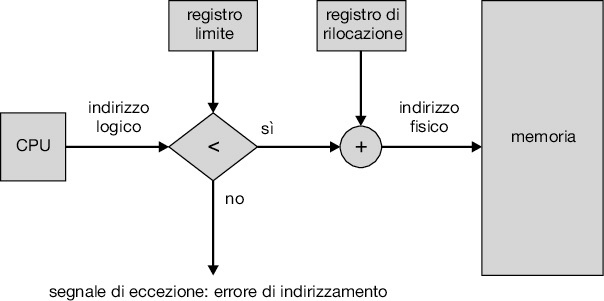
\includegraphics[width=0.5\linewidth]{images/protez_meme.png}
    \caption{Protezione memoria}
    \label{fig:9.6}
\end{figure}

\subsection{Allocazione a partizioni multiple fisse}
Nell'allocazione a partizioni fisse:
\begin{itemize}
    \item La memoria è divisa in \textbf{partizioni di dimensione fissa}, che non devono necessariamente essere tutte uguali.
    \item Ogni partizione contiene un \textbf{unico processo} dall'inizio alla fine della sua esecuzione.
    \item Il \textbf{grado di multiprogrammazione} è determinato dal numero di partizioni.
    \item Quando un processo termina, la partizione può essere occupata da un altro processo.
\end{itemize}

Il meccanismo di \textbf{registri limite e di rilocazione} protegge le partizioni da accessi non autorizzati. Durante il \textit{context switch}, il \textbf{dispatcher} carica:
\begin{itemize}
    \item Nel registro di rilocazione, l'indirizzo di partenza della partizione assegnata al processo.
    \item Nel registro limite, la dimensione della partizione.
\end{itemize}

Questa tecnica, utilizzata nel \textbf{IBM OS/360}, richiede CPU dotate di registri di rilocazione e limite, ma non è più utilizzata nei sistemi operativi moderni per i seguenti svantaggi:
\begin{itemize}
    \item Il grado di multiprogrammazione è limitato dal numero di partizioni disponibili.
    \item Si verifica \textbf{frammentazione interna}, dove una parte della partizione rimane inutilizzata se il processo è più piccolo della partizione stessa.
    \item Si può verificare \textbf{frammentazione esterna}, quando lo spazio libero disponibile è frammentato in più aree non contigue e quindi non utilizzabile per un nuovo processo di dimensione maggiore.
    \item L'arrivo di un processo più grande della partizione più grande non può essere gestito.
\end{itemize}

\textbf{Frammentazione interna}:
\begin{itemize}
    \item Parte dello spazio di memoria di una partizione viene sprecato se il processo è più piccolo della partizione stessa.
\end{itemize}

\textbf{Frammentazione esterna}:
\begin{itemize}
    \item Se la memoria libera è frammentata in più blocchi non contigui, pur avendo spazio sufficiente in totale, non può essere utilizzata per allocare nuovi processi.
\end{itemize}

L’allocazione a partizioni fisse ha anche altri problemi:
\qs{}{Che succede se arriva un processo più grande della partizione più grande?}
\clm{}{}{Notate che se si aumenta la dimensione media delle partizioni, aumenta anche la frammentazione interna, e diminuisce il grado di multiprogrammazione}

\section{Allocazione a partizioni multipli variabili}
Nell'allocazione a partizioni variabili:
\begin{itemize}
    \item Ogni processo riceve una quantità di memoria esattamente pari alla sua dimensione.
    \item Quando un processo termina, lascia un "buco" in RAM che può essere occupato da un altro processo.
    \item Tuttavia, nel tempo si creano \textbf{buchi sparsi e più piccoli}, rendendo difficile l'allocazione di nuovi processi.
\end{itemize}

\begin{figure}[h]
    \centering
    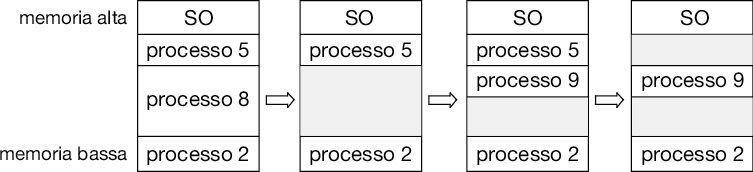
\includegraphics[width=0.5\linewidth]{images/ram_buchi.png}
    \caption{Buchi Ram}
    \label{fig:ram_hole}
\end{figure}
Il sistema operativo (SO) deve:
\begin{itemize}
    \item Tenere traccia delle aree di memoria libere e occupate.
    \item Aggiornare continuamente le informazioni quando un processo nasce o termina.
    \item Assegnare una partizione sufficientemente grande quando un nuovo processo deve essere caricato.
\end{itemize}

\subsection*{Strategie di Allocazione}
Esistono diverse strategie per scegliere quale partizione assegnare a un processo:
\begin{itemize}
    \item \textbf{First Fit}: seleziona la prima partizione abbastanza grande da ospitare il processo.
    \item \textbf{Best Fit}: seleziona la partizione più piccola che può contenere il processo.
    \item \textbf{Worst Fit}: seleziona la partizione più grande disponibile.
\end{itemize}

\textbf{Osservazioni sperimentali}:
\begin{itemize}
    \item La strategia \textbf{Worst Fit} tende a funzionare peggio in termini di utilizzo della memoria, poiché lascia spazi grandi frammentati.
    \item Le strategie \textbf{Best Fit} e \textbf{First Fit} hanno prestazioni simili, ma si preferisce \textbf{First Fit} poiché è più veloce, dato che interrompe la ricerca al primo spazio sufficiente.
\end{itemize}

\subsection{La frammentazione}
Nel tempo, l'allocazione a partizioni variabili può portare alla formazione di piccoli \textbf{buchi non contigui} in RAM:
\begin{itemize}
    \item Circa \textbf{1/3 a 1/2 della memoria principale} (MP) può essere sprecato a causa della \textbf{frammentazione esterna}, ossia la presenza di buchi di memoria troppo piccoli per ospitare un processo.
    \item Esiste anche il problema della \textbf{frammentazione interna}, dovuto all'impossibilità di tenere traccia di buchi molto piccoli che vengono quindi aggregati a partizioni adiacenti, causando uno \textbf{spreco nascosto}.
\end{itemize}

\subsubsection*{Compattazione della Memoria}

Una tecnica per recuperare la memoria inutilizzata è la \textbf{compattazione}:
\begin{itemize}
    \item Spostare le partizioni occupate dai processi in modo che siano tutte \textbf{contigue}, liberando un unico grande buco libero.
    \item La compattazione richiede la \textbf{rilocazione dinamica} del codice e dei dati dei processi.
    \item Questo processo è \textbf{costoso in termini di tempo} e durante la compattazione il sistema non è utilizzabile.
\end{itemize}

\section{Paginazione della memoria}
\dfn{}{
L’allocazione contigua della memoria principale presenta quindi diversi problemi.
L’alternativa è ammettere che l’area di memoria allocata ad un processo possa essere in realtà suddivisa in tanti pezzi non contigui fra loro
Se tutti i “pezzi” hanno la stessa dimensione allora il termine esatto per indicare questa tecnica è: paginazione della memoria (primaria)}

\subsection{Metodo di base}
La \textbf{Memoria Primaria} (o lo \textbf{spazio di indirizzamento fisico}) è suddivisa in unità dette \textbf{frame} (o pagine fisiche), con le seguenti caratteristiche:
\begin{itemize}
    \item I \textbf{frame} sono tutti della stessa dimensione, che è sempre una \textbf{potenza di due} (ad esempio: 512, 1024, 2048, fino a 8192 byte).
    \item Lo spazio di indirizzamento fisico del processo è visto come un \textbf{unico spazio contiguo} di indirizzi, ma nella realtà è suddiviso in \textbf{pagine logiche}, ciascuna di dimensione uguale ai frame fisici.
\end{itemize}

Per eseguire un processo con \textbf{x pagine}:
\begin{itemize}
    \item Il Sistema Operativo (\textbf{SO}) cerca \textbf{x frame} liberi in cui caricare le pagine del processo. Questi frame non devono essere adiacenti e le pagine possono essere caricate in un ordine qualsiasi.
    \item Ogni processo ha una propria \textbf{Tabella delle Pagine} (o \textbf{Page Table}, \textbf{PT}): un array le cui \emph{entry} contengono i numeri dei frame in cui le pagine del processo sono state caricate.
    \item Il SO tiene traccia dei \textbf{frame liberi} nella memoria primaria, utilizzandoli per memorizzare le pagine di nuovi processi.
\end{itemize}

\subsection*{Struttura della Tabella delle Pagine}
\begin{itemize}
    \item Ogni \emph{entry} della Page Table rappresenta una pagina del processo.
    \item L'indice di ciascuna entry corrisponde al numero della pagina, mentre il valore dell'entry contiene il numero del frame dove è stata memorizzata la pagina.
\end{itemize}

\subsection*{Problema degli Indirizzi Virtuali}
Gli \textbf{indirizzi relativi (o virtuali)} del programma, una volta caricati in RAM, non funzionano più come indirizzi lineari contigui. Ad esempio:
\begin{itemize}
    \item Un'istruzione come \texttt{jmp\_if\_odd R1,C} deve saltare a un indirizzo specifico (ad es. 0004), ma in RAM non esiste più un punto lineare di partenza.
    \item La soluzione è \textbf{riconsiderare} gli indirizzi virtuali, non più come indirizzi lineari, ma come indirizzi all'interno della Page Table, utilizzando \textbf{conversioni da indirizzi logici a indirizzi fisici}.
\end{itemize}


Indirizzi Logici e Fisici, vedere registrazione 25/10/2024 min Circa 30
